\documentclass[aspectratio=169,11pt]{beamer}

\usepackage{graphicx}
\usepackage{tikz}
\usetikzlibrary{positioning,arrows.meta}
\usepackage{xcolor}
\usepackage{booktabs}
\usepackage{tabularx}
\usepackage{array}
\usepackage{ragged2e}

\definecolor{GEUBlue}{RGB}{20,55,105}
\definecolor{GEULightBlue}{RGB}{238,244,251}
\definecolor{GEUGrey}{RGB}{90,90,90}
\definecolor{GEULightGrey}{RGB}{245,246,248}

\usetheme{default}
\setbeamertemplate{navigation symbols}{}
\setbeamertemplate{blocks}[rounded][shadow=false]
\setbeamercolor{normal text}{fg=black,bg=white}
\setbeamercolor{frametitle}{fg=GEUBlue}
\setbeamercolor{structure}{fg=GEUBlue}
\setbeamercolor{block title}{fg=GEUBlue,bg=GEULightBlue}
\setbeamercolor{block body}{fg=black,bg=GEULightBlue}
\setbeamerfont{frametitle}{size=\Large,series=\bfseries}

% Replace with the actual logo filename
\newcommand{\GEULogo}{logo.jpeg}

% Header and footer
\setbeamertemplate{headline}{%
  \begin{tikzpicture}[remember picture,overlay]
    \node[anchor=north east,xshift=-0.30cm,yshift=-0.12cm]
      at (current page.north east)
      {\includegraphics[height=0.62cm]{\GEULogo}};
  \end{tikzpicture}
  \vspace{0.72cm}
}
\setbeamertemplate{frametitle}{%
  \vspace{0.03cm}
  \insertframetitle\par
  \vspace{0.04cm}
  \textcolor{GEUBlue}{\rule{\textwidth}{0.9pt}}
  \vspace{0.03cm}
}
\setbeamertemplate{footline}{%
  \leavevmode
  \hbox{%
  \begin{beamercolorbox}[wd=.82\paperwidth,ht=0.32cm,dp=0.10cm,leftskip=.3cm]{author in head/foot}
    \tiny Department of Computer Science \& Engineering | Graphic Era (Deemed to be University)
  \end{beamercolorbox}%
  \begin{beamercolorbox}[wd=.18\paperwidth,ht=0.32cm,dp=0.10cm,rightskip=.3cm]{date in head/foot}
    \hfill\tiny\insertframenumber/\inserttotalframenumber
  \end{beamercolorbox}}
}

\newcommand{\smallnote}[1]{\vspace{0.08cm}{\scriptsize\color{GEUGrey}#1}}
\newcommand{\placeholder}[1]{\textit{\color{GEUGrey}#1}}

\title{\textbf{Project-Based Learning}\\[2mm]\large Phase-II Evaluation}
\author{\textbf{RideSync: A Graph-Based Smart Cab Booking and Dispatch Simulation System}\\Team ID: DSCPP-III-2026-T151}
\institute{Department of Computer Science \& Engineering\\Graphic Era (Deemed to be University), Dehradun}
\date{Academic Session 2026--27}

\begin{document}

% 1. Title Slide
\begin{frame}[plain]
\begin{tikzpicture}[remember picture,overlay]
\draw[GEUBlue,line width=3pt] (current page.north west) -- (current page.north east);
\node[anchor=north east,xshift=-0.45cm,yshift=-0.35cm] at (current page.north east)
{\includegraphics[height=1.0cm]{\GEULogo}};
\node[align=center,text width=.84\paperwidth] at ([yshift=.25cm]current page.center)
{{\color{GEUBlue}\fontsize{24}{28}\selectfont\bfseries PROJECT-BASED LEARNING}\\[2mm]
 {\fontsize{16}{20}\selectfont PHASE-II EVALUATION}\\[5mm]
 {\color{GEUGrey}\large\bfseries RideSync: A Graph-Based Smart Cab Booking and Dispatch Simulation System}\\[2mm]
 {\color{GEUBlue}\small Team ID: DSCPP-III-2026-T151}};
\node[align=center,anchor=south,yshift=.42cm] at (current page.south)
{\bfseries Department of Computer Science \& Engineering\\
Graphic Era (Deemed to be University), Dehradun\\[-1mm]
\scriptsize Academic Session 2026--27};
\end{tikzpicture}
\end{frame}

% 2. Team & Mentor Details
\begin{frame}{Team \& Mentor Details}
\small
\vspace{-2mm}
\begin{columns}[T,totalwidth=\textwidth]

\column{.48\textwidth}
\begin{block}{Team Information}
\begin{tabular}{@{}p{2.2cm}p{4.3cm}@{}}
\textbf{Team ID:} & DSCPP-III-2026-T151\\
\textbf{Semester:} & 3rd\\
\textbf{Team Name:} & The Four Bytes\\
\textbf{Domain:} & Data Structures and\\
                 & Programming in C++
\end{tabular}
\end{block}

\column{.48\textwidth}
\begin{block}{Team Members}
\footnotesize
1.\quad Gupta, Tanvi -- 2510010362 (Team Lead)\\
2.\quad Jahnavi -- 2510380066\\
3.\quad Tyagi, Nishtha -- 2510370096\\
4.\quad Sharma, Dhairya -- 2510011490
\end{block}

\end{columns}

\vspace{1mm}

\begin{block}{Mentor}
\footnotesize
\placeholder{Dr. Hemant Singh Pokhariya (hemantsinghpokhariya@geu.ac.in)}
\hfill
\textbf{Interactions completed: 7}
\end{block}

\end{frame}

% 3. Phase-II Abstract & Updated Approach
\begin{frame}{Phase-II Abstract \& Core Approach}

\vspace{-3mm}

\begin{block}{Project Abstract}
\scriptsize
RideSync is a console-based Cab Booking System in C++17. City locations and roads are modelled as weighted graphs, shortest routes are computed using Dijkstra's Algorithm, and driver assignments are optimised through a priority queue using composite scoring. Persistent storage relies on flat text files ($fstream$).
\end{block}

\vspace{1mm}

\begin{columns}[T,totalwidth=\textwidth]

\column{.48\textwidth}
\textbf{\color{GEUBlue}Architecture Highlights}
\begin{itemize}\itemsep1pt
\item \footnotesize Encapsulated classes: Customer, Driver, Cab, Admin, and Booking
\item \footnotesize Auth Manager handles user login roles
\item \footnotesize Adjacency list map representation: \texttt{unordered\_map<int, vector<pair<int, int>>>}
\item \footnotesize STL stack for recent booking history
\end{itemize}

\column{.48\textwidth}
\textbf{\color{GEUBlue}Design Choices}
\begin{itemize}\itemsep1pt
\item \footnotesize Modular layout with separate headers and source implementation files
\item \footnotesize Predefined city location mappings (no live GPS dependency)
\item \footnotesize Input validation to prevent crashes from invalid IDs or out-of-service cabs
\end{itemize}

\end{columns}

\end{frame}

% 4. Tasks Completed in Phase-II
\begin{frame}{Phase-II Progress: Tasks Completed}

\footnotesize
\vspace{-2mm}
\textbf{\color{GEUBlue}Completed Milestones \& Contributions}
\vspace{1mm}

\begin{itemize}\itemsep2pt
\item \textbf{Problem Definition \& System Design (Phase 1):} Completed collectively by all team members.
\item \textbf{Object-Oriented Structure:} Designed base classes and derived structures (Customer, Driver, Cab, Admin, User, AuthManager) by Tanvi Gupta \& Nishtha Tyagi.
\item \textbf{Authentication Module:} Implemented secure user login, credential verification, and role management by Tanvi Gupta \& Nishtha Tyagi.
\item \textbf{Graph Engine \& Dispatch Logic Framework:} Initial architectural planning for City Graph, Dijkstra's route engine and Driver Dispatch priority queue formulation (Jahnavi).
\end{itemize}

\vspace{1mm}
\begin{center}
\colorbox{GEULightBlue}{%
\parbox{0.90\textwidth}{%
\centering
\scriptsize
\textbf{Status:} Core OOP architecture and authentication modules fully implemented; algorithmic modules progressing according to schedule.%
}}
\end{center}

\end{frame}

% 10. RideSync Website: Interface Preview
\begin{frame}{RideSync Website: Interface Preview}

\vspace{-3mm}
\centering

\setlength{\fboxsep}{2pt}
\setlength{\fboxrule}{0.8pt}

% Row 1
\begin{minipage}[t]{0.42\textwidth}
    \centering
    \fcolorbox{GEUBlue}{white}{%
        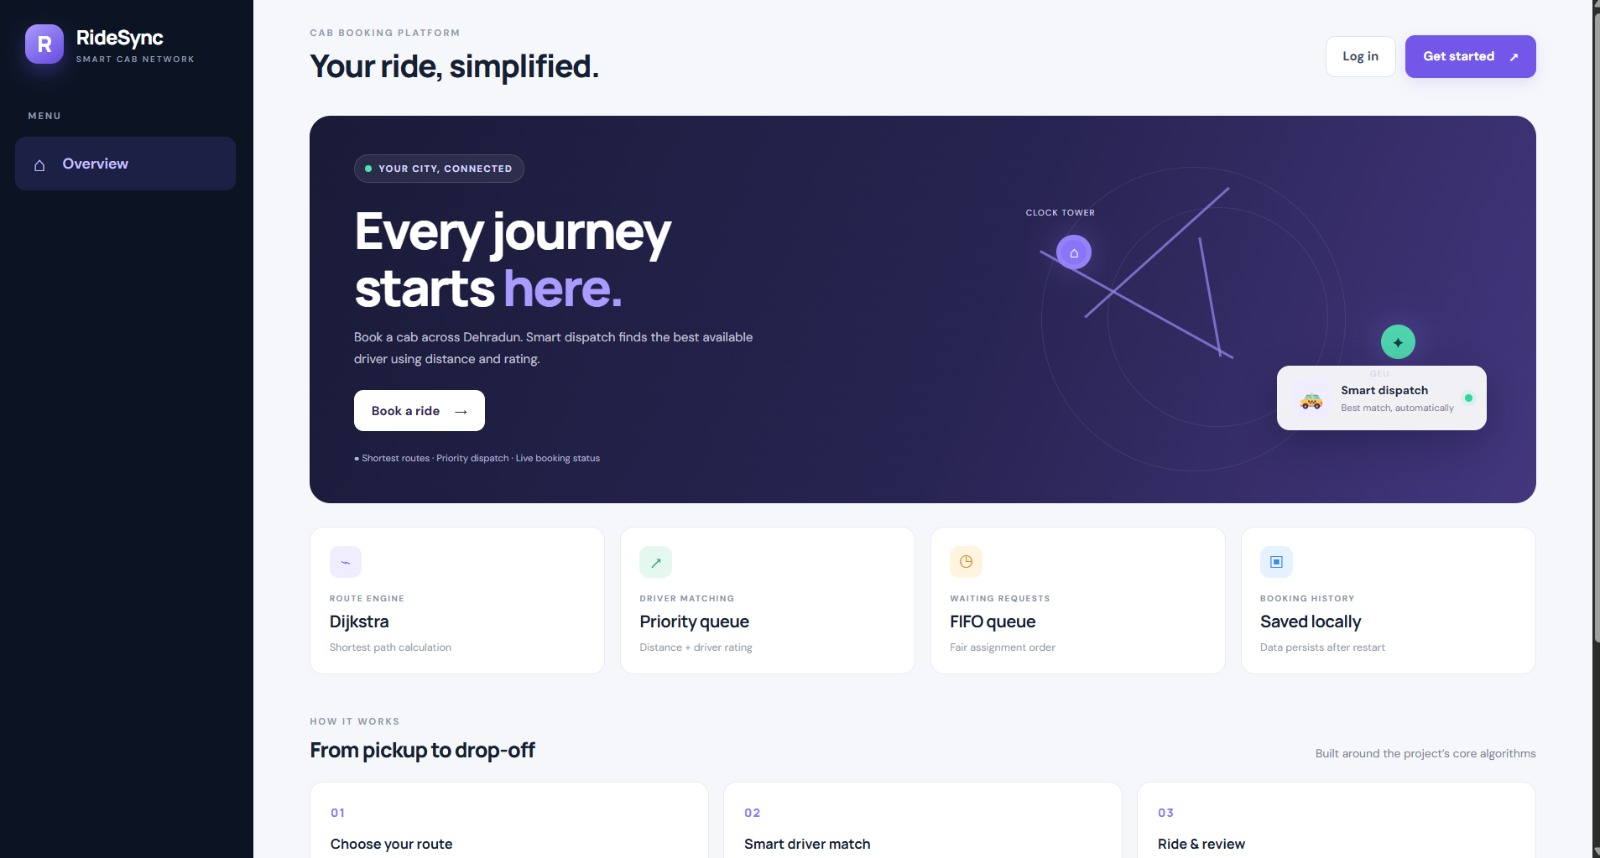
\includegraphics[
            width=\dimexpr\linewidth-8\fboxsep-6\fboxrule\relax,
            height=0.29\textheight,
            keepaspectratio
        ]{hp.jpeg}
    }\\[1mm]
    {\scriptsize\bfseries\color{GEUBlue}Homepage}
\end{minipage}
\hfill
\begin{minipage}[t]{0.42\textwidth}
    \centering
    \fcolorbox{GEUBlue}{white}{%
        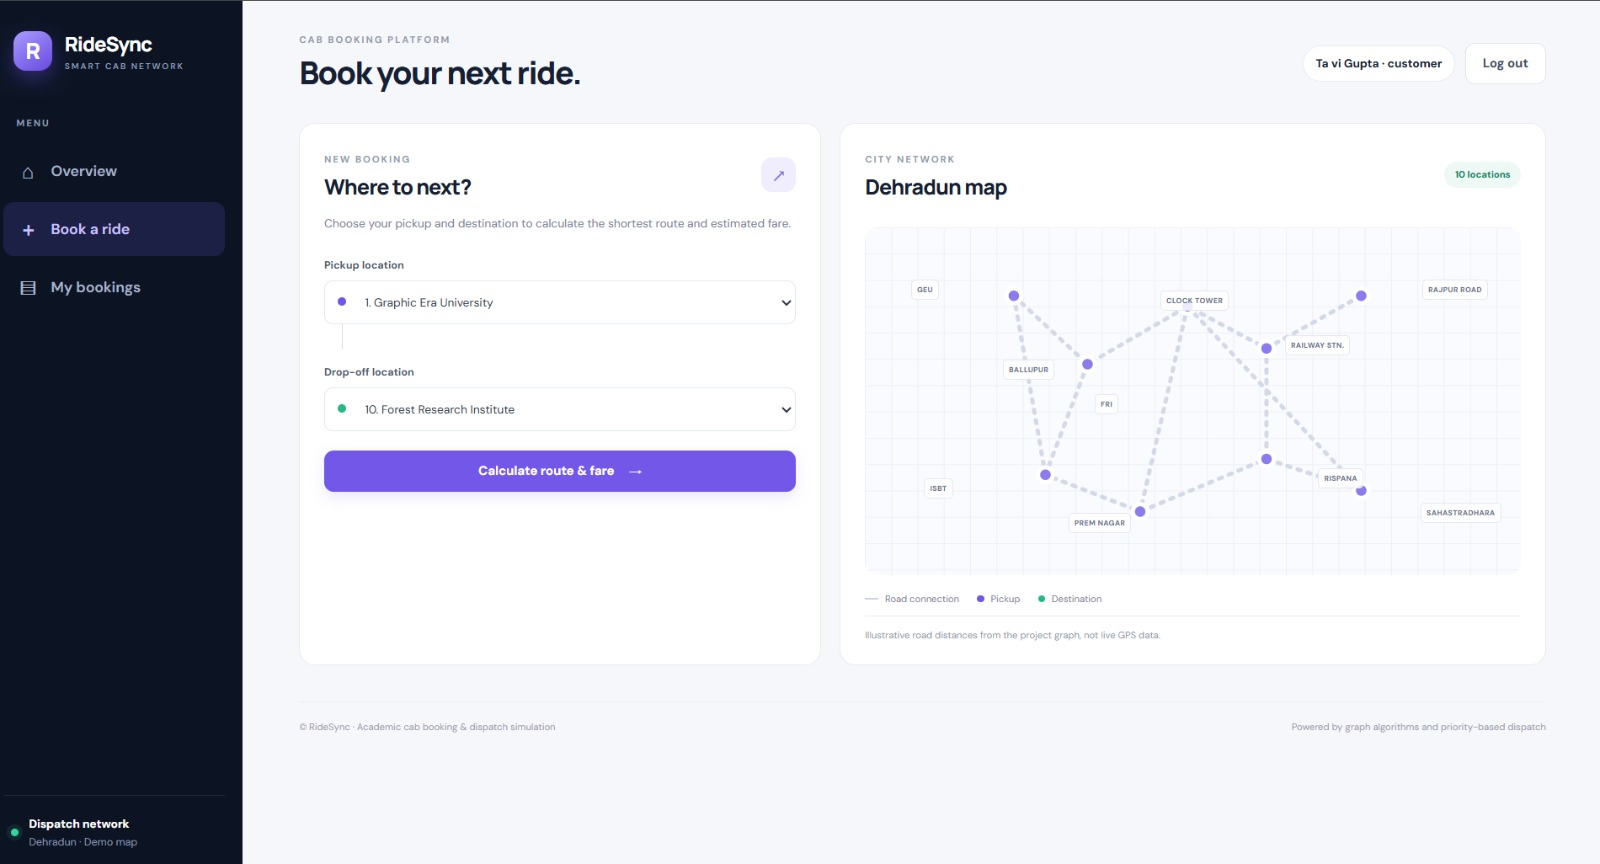
\includegraphics[
            width=\dimexpr\linewidth-2\fboxsep-2\fboxrule\relax,
            height=0.29\textheight,
            keepaspectratio
        ]{cp.jpeg}
    }\\[1mm]
    {\scriptsize\bfseries\color{GEUBlue}Booking Interface}
\end{minipage}

\vspace{2mm}

% Row 2
\begin{minipage}[t]{0.42\textwidth}
    \centering
    \fcolorbox{GEUBlue}{white}{%
        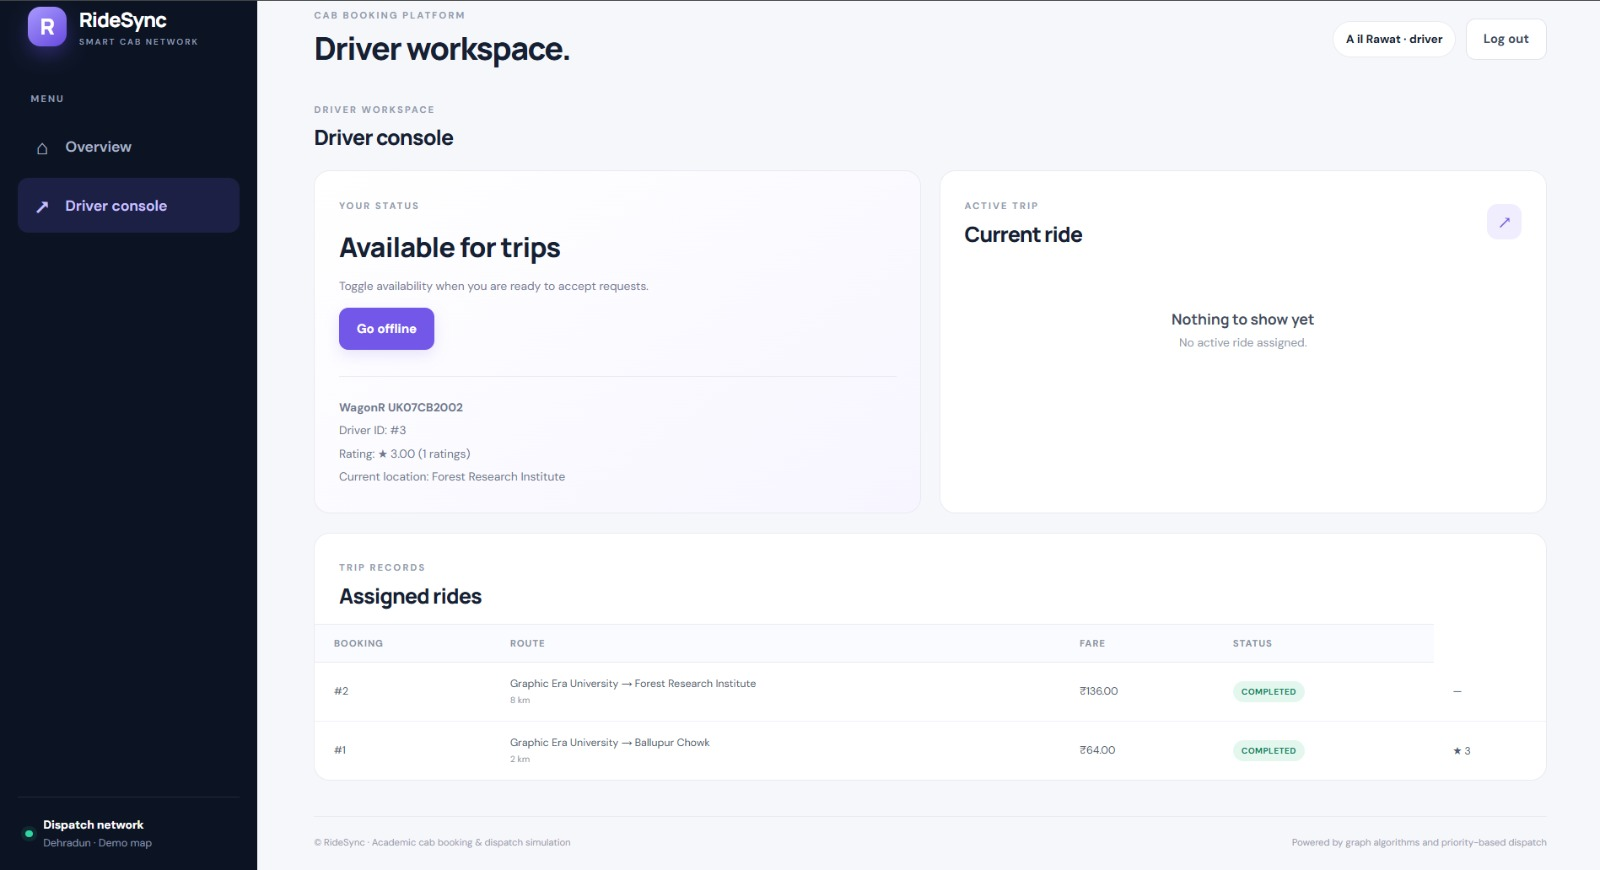
\includegraphics[
            width=\dimexpr\linewidth-2\fboxsep-2\fboxrule\relax,
            height=0.29\textheight,
            keepaspectratio
        ]{dr.jpeg}
    }\\[1mm]
    {\scriptsize\bfseries\color{GEUBlue}Driver Console}
\end{minipage}
\hfill
\begin{minipage}[t]{0.42\textwidth}
    \centering
    \fcolorbox{GEUBlue}{white}{%
        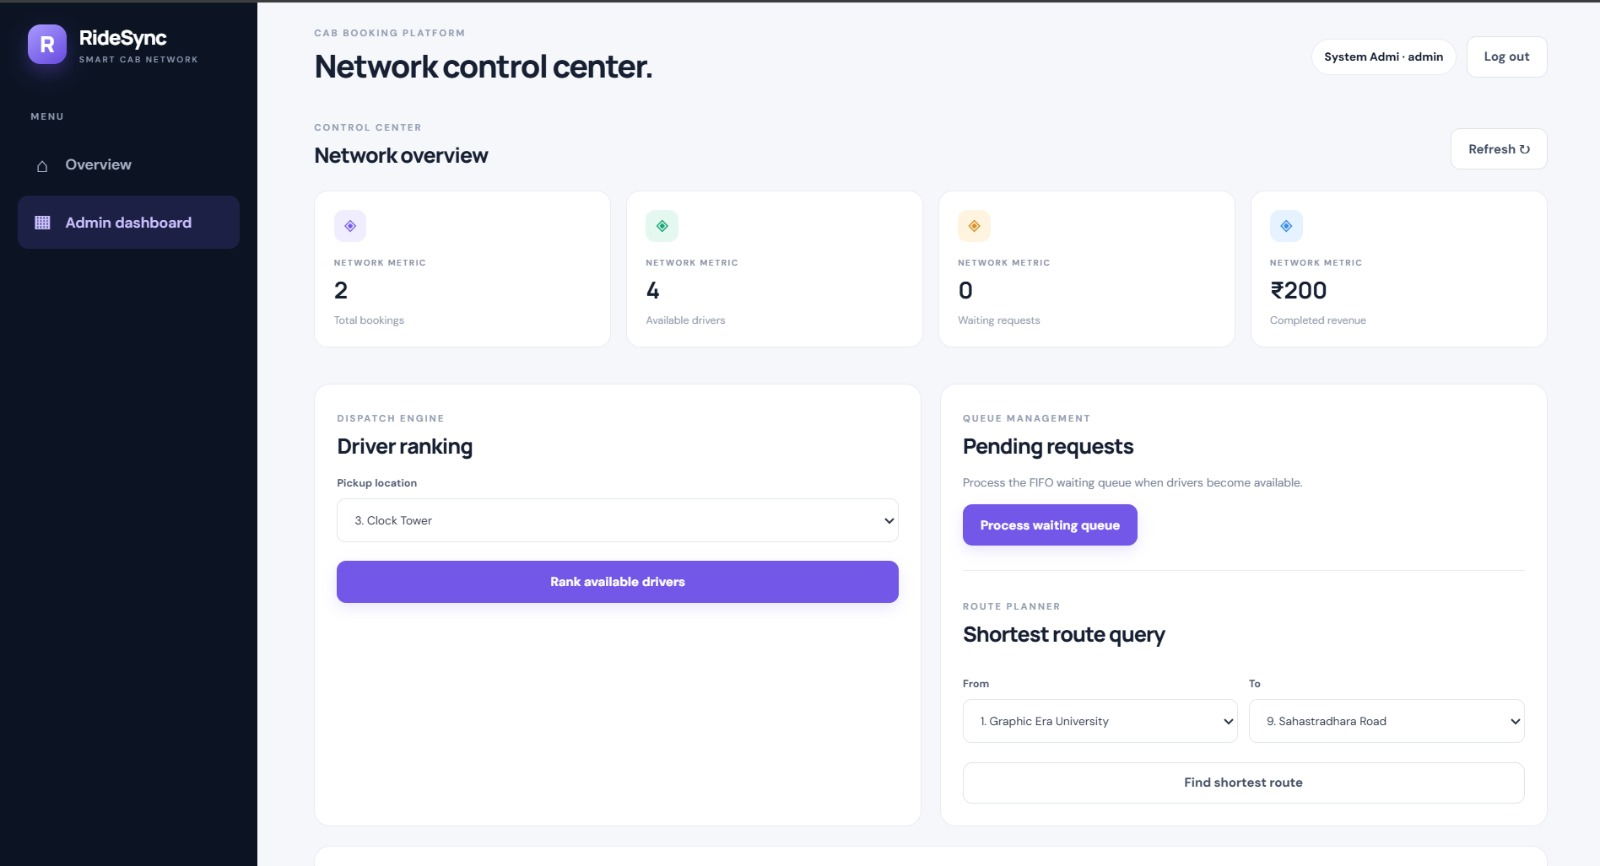
\includegraphics[
            width=\dimexpr\linewidth-2\fboxsep-2\fboxrule\relax,
            height=0.29\textheight,
            keepaspectratio
        ]{ad.jpeg}
    }\\[1mm]
    {\scriptsize\bfseries\color{GEUBlue}Admin Dashboard}
\end{minipage}

\end{frame}


% 5. Current Challenges & Roadblocks Addressed
\begin{frame}{Challenges \& Technical Roadblocks}

\footnotesize
\vspace{-2mm}

\begin{columns}[T,totalwidth=\textwidth]

\column{.48\textwidth}
\textbf{\color{GEUBlue}Challenges Encountered}
\begin{enumerate}\itemsep1pt
\item \textbf{Module Integration:} Coordinating equal workload distribution across four members via structured GitHub commits and modular header/source files.
\item \textbf{Robust Validation:} Preventing console application crashes from invalid location IDs or out-of-service cab inputs.
\end{enumerate}

\column{.48\textwidth}
\textbf{\color{GEUBlue}Solutions Implemented}
\begin{enumerate}\itemsep1pt
\item \textbf{Composite Dispatch Score:} Formulated and tested custom weightings combining physical distance and driver rating for the priority queue max-heap.
\item \textbf{Pre-Integration Unit Testing:} Rigorously unit-testing individual components prior to merging into the central \texttt{main.cpp} integration workflow.
\end{enumerate}

\end{columns}

\vspace{2mm}
\begin{center}
\tiny
\textit{Repository: \texttt{github.com/TanviGupta12/RideSync-Cab-Booking-Dispatch} (Branch: \texttt{main})}
\end{center}

\end{frame}

% 6. Integration of PBL Course Concepts
\begin{frame}{Integration of PBL Course Concepts}
\tiny
\begin{center}
\renewcommand{\arraystretch}{1.2}
\begin{tabularx}{.96\textwidth}{@{}>{\bfseries}p{3.5cm}X p{2.2cm}@{}}
\toprule
Course/Area & Concepts Applied & Project Module\\
\midrule
Data Structures \& Algorithms & Graph, Priority Queue, Stack, Linked List, Dijkstra's Algorithm, Searching, Sorting & Routing, Driver Assignment \& Booking History\\
OOP with C++ & Classes \& Objects, Constructors, Inheritance, Polymorphism, Encapsulation, STL, File Handling & Customer, Driver, Cab, Admin \& Booking\\
\bottomrule
\end{tabularx}
\end{center}

\vspace{2mm}

\begin{center}
\colorbox{GEULightBlue}{\parbox{.86\textwidth}{\centering
\scriptsize \textbf{Phase-II Update:} Successfully combining advanced C++ STL containers (\texttt{vector}, \texttt{priority\_queue}, \texttt{unordered\_map}, \texttt{stack}) with robust OOP design patterns.}}
\end{center}
\end{frame}

% 7. System Architecture & Codebase Status
\begin{frame}{Codebase \& Component Status}

\vspace{-4mm}

\begin{center}
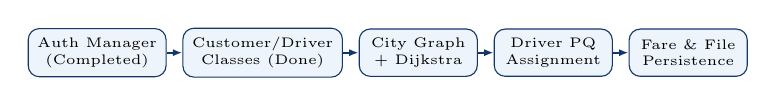
\begin{tikzpicture}[
node distance=2mm,
box/.style={
rectangle,
rounded corners,
draw=GEUBlue,
fill=GEULightBlue,
minimum width=1.5cm,
minimum height=6mm,
align=center,
font=\tiny
},
arrow/.style={
-{Latex[length=1.2mm]},
thick,
draw=GEUBlue
}
]

\node[box] (a) {Auth Manager\\(Completed)};
\node[box,right=of a] (b) {Customer/Driver\\Classes (Done)};
\node[box,right=of b] (c) {City Graph\\+\ Dijkstra};
\node[box,right=of c] (d) {Driver PQ\\Assignment};
\node[box,right=of d] (e) {Fare \& File\\Persistence};

\draw[arrow] (a)--(b);
\draw[arrow] (b)--(c);
\draw[arrow] (c)--(d);
\draw[arrow] (d)--(e);

\end{tikzpicture}
\end{center}

\vspace{0mm}

\begin{columns}[T,totalwidth=\textwidth]

\column{.48\textwidth}
\textbf{\color{GEUBlue}\tiny Key Commits \& Contributions}
\begin{itemize}\itemsep0.5pt
\item \tiny \textbf{Tanvi Gupta:} Architecture, Auth, fare, file logging, CLI
\item \tiny \textbf{Jahnavi:} CityGraph adjacency list \& Dijkstra routing
\item \tiny \textbf{Nishtha Tyagi:} Derived classes, location, stack history

\end{itemize}

\column{.48\textwidth}
\textbf{\color{GEUBlue}\tiny Testing \& Validation Status}
\begin{itemize}\itemsep0.5pt
\item \tiny \textbf{Unit Testing:} In progress for components prior to integration
\item \tiny \textbf{Input Validation:} Scheduled for error handling on invalid IDs
\item \tiny \textbf{Integration Testing:} Planned for Phase 5
\end{itemize}

\end{columns}

\end{frame}

% 8. Technology Stack & Methodology
\begin{frame}{Technology Stack \& Methodology}

\footnotesize
\vspace{-3mm}

\begin{columns}[T,totalwidth=\textwidth]

\column{.55\textwidth}
\begin{block}{Technology Stack}
\tiny
\begin{itemize}\itemsep0.5pt
\item Language: C++17
\item STL Containers: vector, queue, priority\_queue, unordered\_map, stack
\item Core Concepts: OOP, Encapsulation, Inheritance, Polymorphism
\item Algorithms: Dijkstra's Shortest Path, Priority Queue Max-Heap
\item Persistence: Flat text files via \texttt{fstream}
\item Tools: VS Code, GitHub Version Control
\end{itemize}
\end{block}

\column{.41\textwidth}
\begin{block}{Development Methodology}
\tiny
\begin{enumerate}\itemsep0.5pt
\item Problem Definition (\textit{Done})
\item Requirement Analysis (\textit{Done})
\item System Design (\textit{Done})
\item Class Design \& Auth (\textit{Done})
\item Algorithm Integration (\textit{In Progress})
\item File Persistence \& Testing (\textit{Pending})
\end{enumerate}
\end{block}

\end{columns}

\end{frame}

% 9. Pending Tasks & Future Roadmap
\begin{frame}{Pending Tasks \& Roadmap}

\tiny
\vspace{-5mm}

\begin{columns}[T,totalwidth=\textwidth]

\column{.64\textwidth}
\textbf{\color{GEUBlue}Pending Tasks Allocation}

\begin{enumerate}
\setlength{\itemsep}{0.5pt}
\setlength{\parskip}{0pt}
\item \textbf{Graph Representation :} Jahnavi
\item \textbf{Resolve code errors:} Dhairya Sharma
\item \textbf{File Handling (\texttt{fstream}) Persistence:} Tanvi Gupta \& Nishtha 
\item \textbf{Deployment of Website:} Dhairya Sharma
\item \textbf{End-to-End Testing:} All team members
\end{enumerate}

\vspace{1mm}

\textbf{\color{GEUBlue}Execution Roadmap}

\begin{enumerate}
\setlength{\itemsep}{0.5pt}
\setlength{\parskip}{0pt}
\item Phase 1: Problem Statement \& Proposed Solution (\textit{Completed})
\item Phase 2: Core Code Implementation (\textit{70\% Completed})
\item Phase 3: Debugging, File Handling \& End-to-End Testing (\textit{Pending})
\end{enumerate}


\column{.34\textwidth}
\textbf{\color{GEUBlue}References}

\begin{enumerate}
\setlength{\itemsep}{0.5pt}
\setlength{\parskip}{0pt}
\item cppreference.com -- C++17 Library
\item GeeksforGeeks -- OOP in C++
\item GeeksforGeeks -- Dijkstra's Algorithm
\item cplusplus.com -- STL Containers
\item cplusplus.com -- File Handling
\end{enumerate}

\vspace{2mm}

\begin{center}
\colorbox{GEUBlue}{%
\parbox{.98\linewidth}{%
\centering
\color{white}
\textbf{Thank You}\\[-1pt]
Regards!
}}
\end{center}

\end{columns}

\end{frame}

\end{document}